\section{Arkitektur}

Der er i projektet brugt en lagdelt 3-tier arkitektur, der består af \textbf{Presentation layer} i Next.js, \textbf{Application layer}
i Express, Graphql og med business logic, og \textbf{Data layer} i en Postgres database.
Den er opdelt i en Client side og en Server side.

\subsection{Presentation Layer}
Frontend-laget er implementeret i Next.js og fungerer som brugerens interface med systemet.
Her håndteres brugerinteraktioner, formularer og visning af data fra GraphQL API'et.
Vi bruger server-side rendering for at optimere load-tider på sider med mange data,
og state management sker via React's useState og context API.

\subsection{Application Layer}
Backend-laget består af en Node.js server med Express og GraphQL.
GraphQL fungerer som API-lag, hvor resolvers håndterer queries og mutationer
og kommunikerer med service-laget, der implementerer business logic.
Middleware håndterer authentication, logging og error handling.

\subsection{Data Layer}
Databasen er en PostgreSQL-server, hvor vores data er modelleret som vist på Figur~\ref{fig:ER-diagram}.
Vi har normaliseret tabellerne til 3NF for at undgå redundans, og constraints sikrer dataintegritet.
Data-laget er isoleret fra klienten og tilgås udelukkende gennem applikationslaget.

\begin{figure}[h!]
    \centering
    \fbox{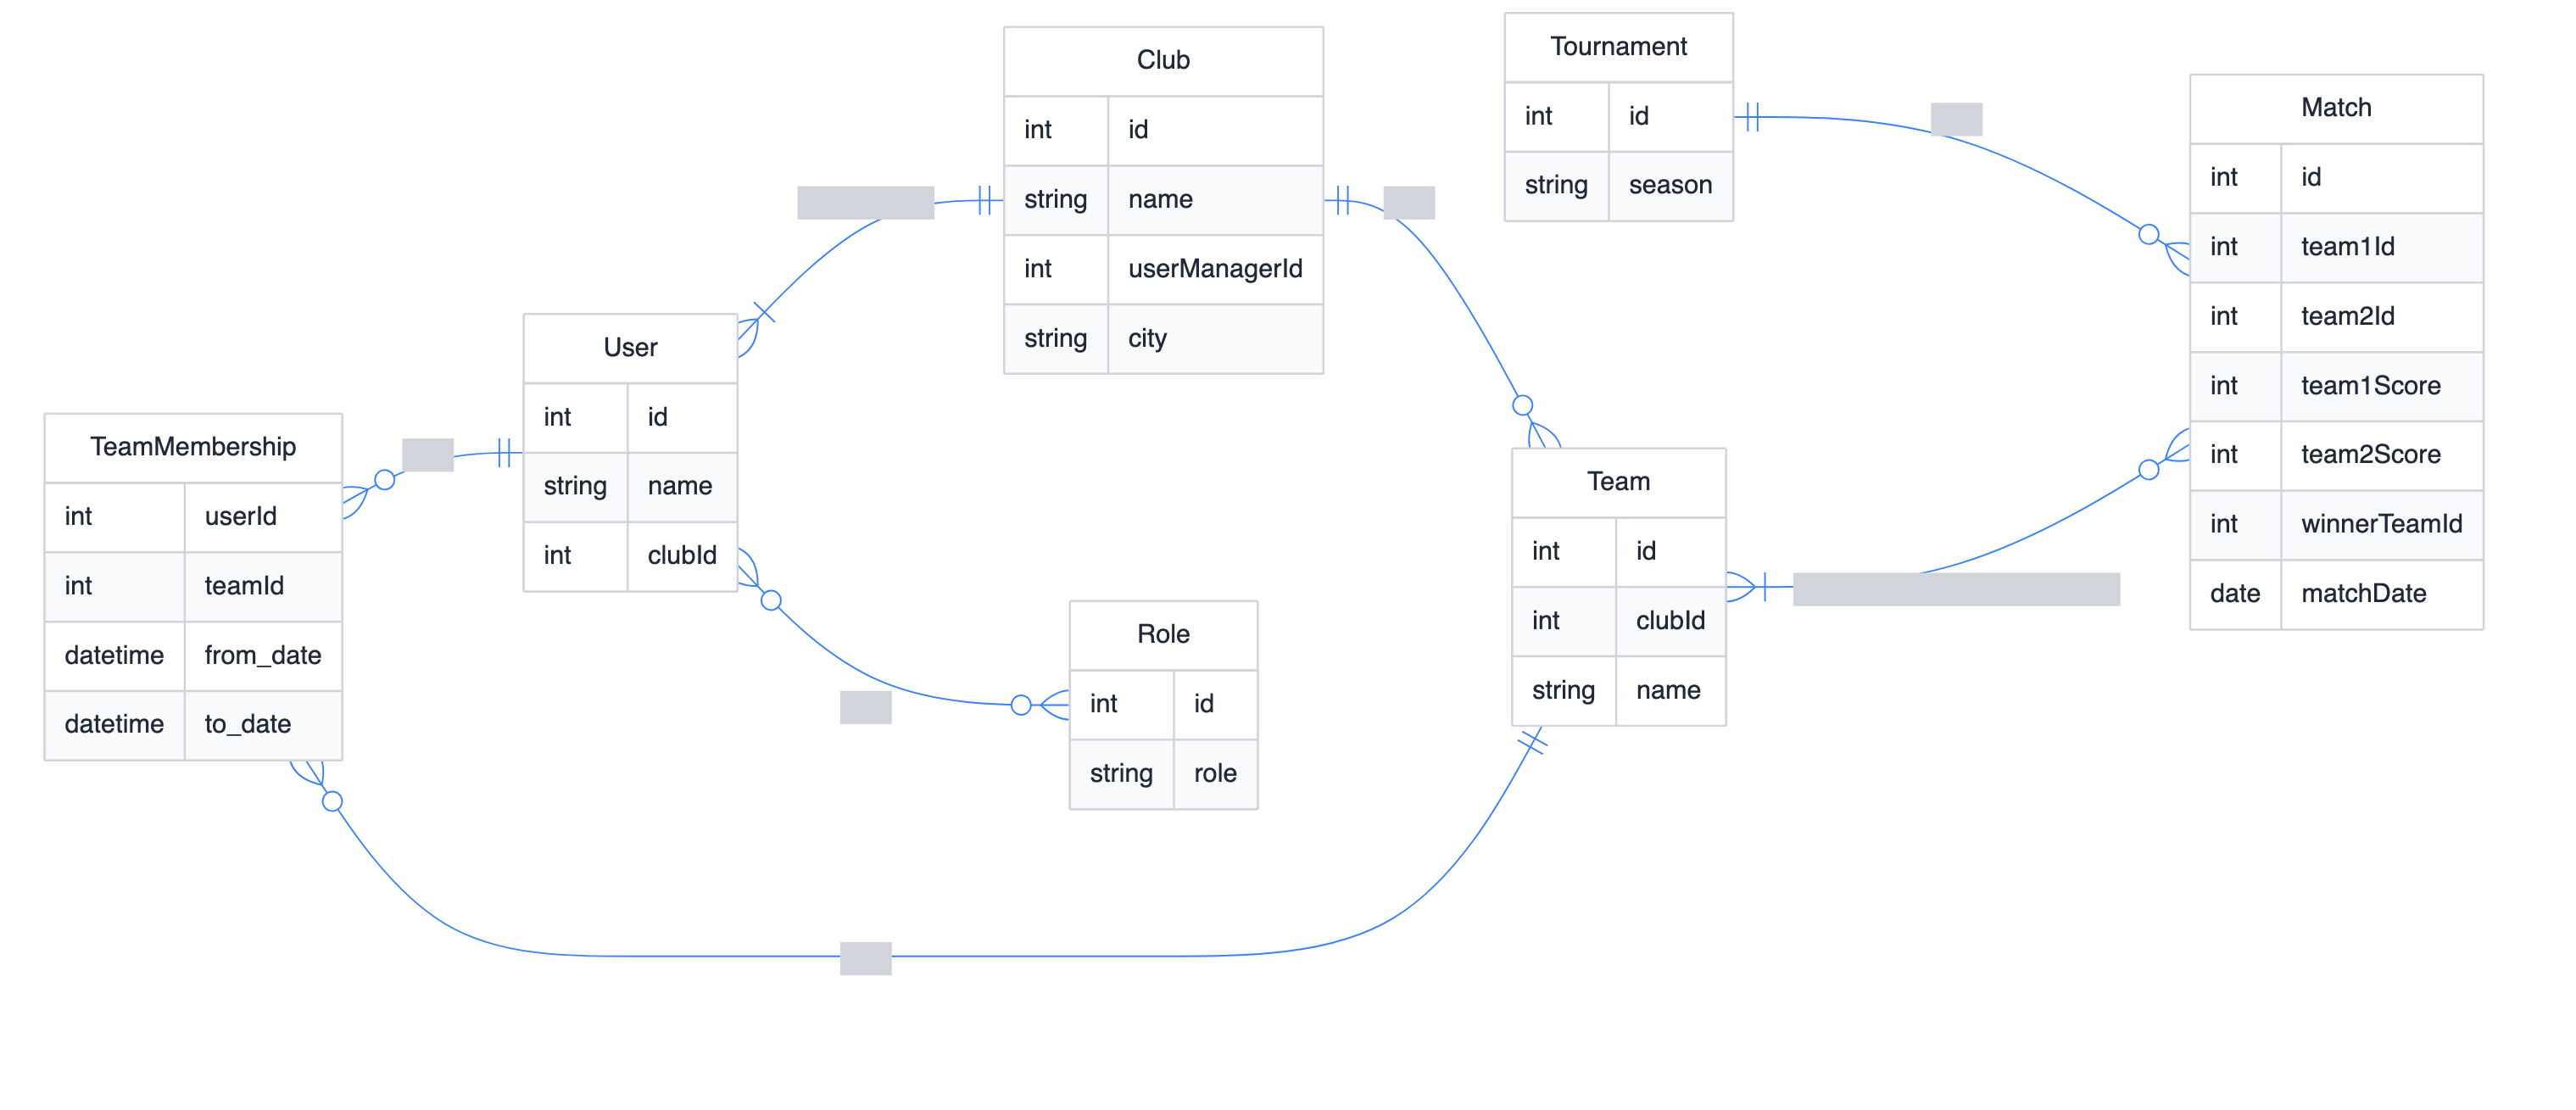
\includegraphics[width=1\textwidth]{Dokumenter/bilag/Diagrammer/ER-diagram}}
    \caption{ER-diagram}
    \label{fig:ER-diagram}
\end{figure}